\section{Bevölkerungsdichten der Landkreise und Regierungsbezirke}
In \autoref{fig:distribution_pop_density_counties} sind die Bevölkerungsdichten der einzelnen Landkreise dargestellt. Auf der linken Seite befindet sich die Verteilung und auf der rechten Seite die räumliche Anordnung.

Die Bezirke Berlins sind einzeln gelistet, daher entsprechen die sechs höchsten Bevölkerungsdichten den Berliner Bezirken  Friedrichshain-Kreuzberg, Mitte, Neukölln, Tempelhof-Schöneberg, Lichtenberg, Charlottenburg-Wilmersdorf, obwohl die Bevölkerungsdichte des gesamten Berliner Stadtkreises niedriger ist als die Bevölkerungsdichte Münchens. In dieser Auflistung ist München Platz 7, fasst man die Berliner Bezirke zusammen, liegt München auf Platz 1.

\begin{figure}[H]
    \centering
    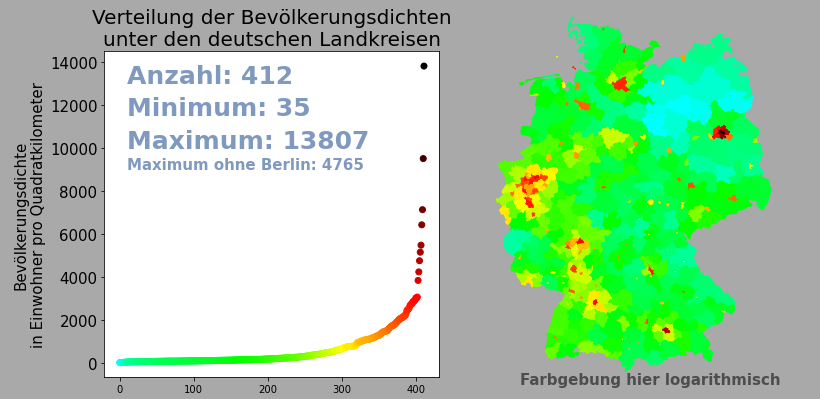
\includegraphics[width = 0.95\textwidth]{figures/Ergebnisse/population_density_counties.png}
    \caption{Verteilung der Bevölkerungsdichten unter den deutschen Landkreisen.}
    \label{fig:distribution_pop_density_counties}
\end{figure}

In \autoref{fig:distribution_pop_density_districts} sind die Bevölkerungsdichten der einzelnen Regierungsbezirke dargestellt. Auf der linken Seite befindet sich die Verteilung und auf der rechten Seite die räumliche Anordnung.

\begin{figure}[H]
    \centering
    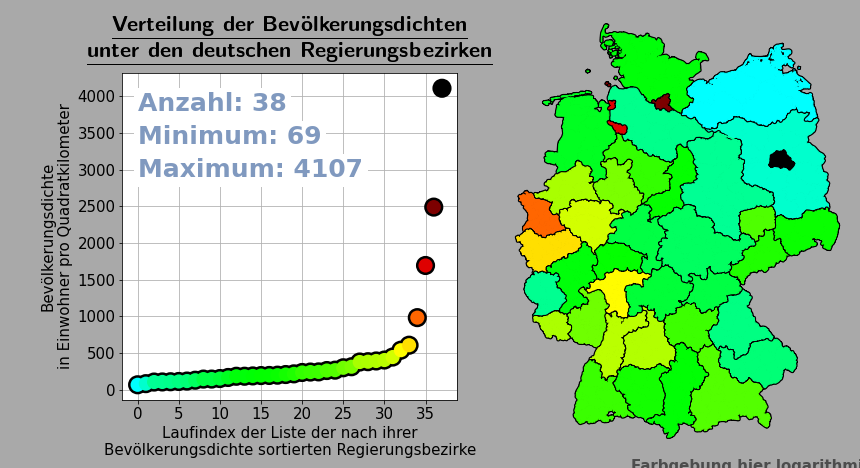
\includegraphics[width = 0.95\textwidth]{figures/Ergebnisse/population_density_ditricts.png}
    \caption{Verteilung der Bevölkerungsdichten unter den deutschen Regierungsbezirken. Die Skalierung entspricht der Farbgebung in \autoref{fig:distribution_pop_density_counties}.}
    \label{fig:distribution_pop_density_districts}
\end{figure}